While there are several proposals for disaggregated WSCs, we will use the
Firebox\cite{firebox} project as an example throughout this thesis (see figure
\ref{fig:fb_diagram}).

\begin{figure}
    \centering
    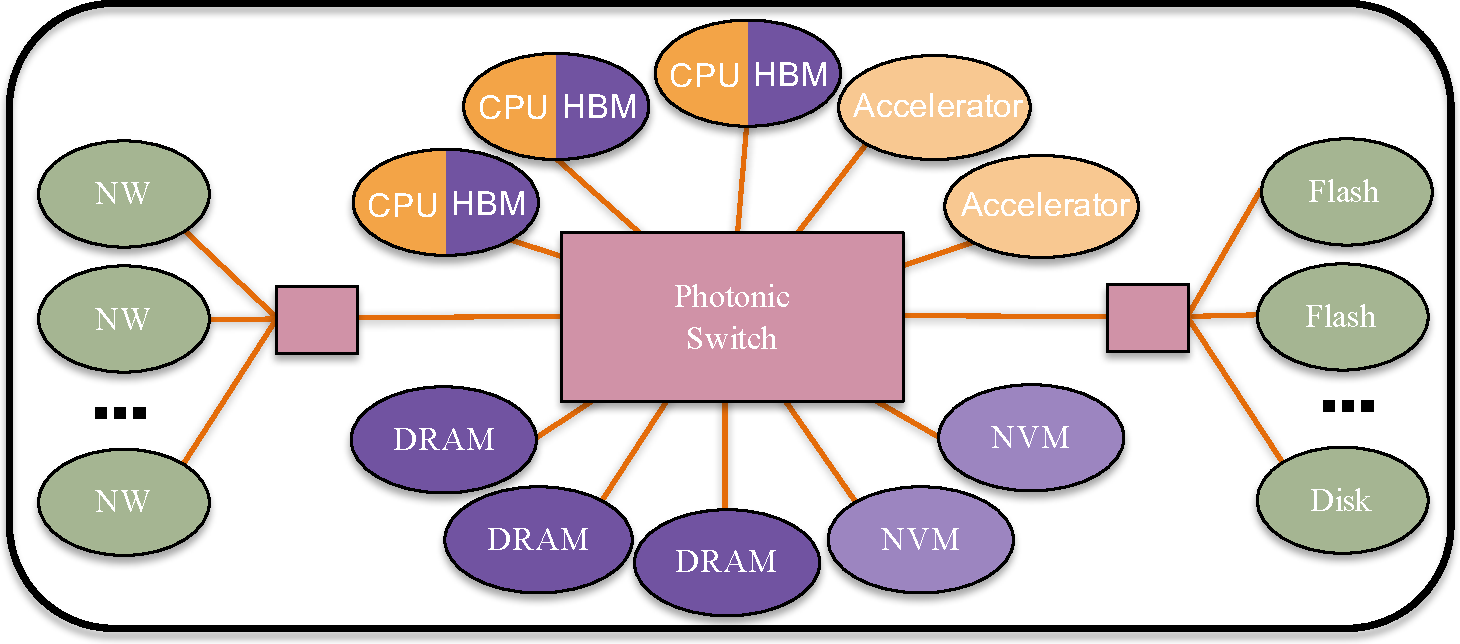
\includegraphics[width=0.9\columnwidth]{figs/FBDiagram.pdf} \label{fig:fb_diagram}
    \vspace{-5mm}
    \caption{The Firebox WSC}
\end{figure}

Firebox proposes using high-bandwidth, high-radix, silicon photonic networks to
connect compute, memory, and storage nodes in a WSC. Silicon photonic network
interfaces can be integrated directly into the SiPs, minimizing pin-out and
providing high bandwidth at low power. By multiplexing many wavelengths onto a
single fiber (wave-division multiplexing), it is possible to create a very high
fanout while using few physical interfaces. This fanout may enable very high
radix switches that can connect many SiPs within a single hop. Current
estimates indicate these photonic networks can acheive aggregate bandwidths
exceeding \SI{1}{\tera\bit\per\second} over 128 channels on a single
fiber\cite{naturePhotonic}\cite{Photonic09}. Link latencies (including photonic
transceiver crossings) are on the order of 10s of
\si{\nano\second}, but final latencies will
be determined by protocol decisions. We beleive round-trip latencies (across a
single switch) of approximately \SI{1}{\micro\second} to be a conservative prediction. For
reference, current infiniband EDR networks provide approximately
\SI{24}{\giga\bit\per\second} per
link (with up to 12 links per NIC), and have round-trip latencies of
approximately \SI{2}{\micro\second}\cite{binnigNW}.

Compute nodes can be CPUs or special-purpose accelerators. In either case, they
will include some amount of high-bandwidth on-package memory (HBM), we
typically assume densities of approximately \SI{2}{\giga\byte} per core. The bulk of the memory
in the system will consist of dedicated memory blades which are optimized for
cost, power, and density. The total available memory may be as much as
\SI{1}{\peta\byte}.
Other resources may also be used, such as high-performance NAND flash, disks,
and external network bridges. Ultimately, the scale of such a system will be
limited by network capacity, but a Firebox would include at least thousands of
cores and hundreds of \si{\tera\byte} of bulk memory.
